\section{Semi-Infinite Uniform Source}
This case is also simply an evaluation of an analytic function, but can't be exactly represented by a basis polynomial.  The solution models the mono-energetic neutron flux at a point inside a 1D semi-infinite homogenous absorbing medium with a uniform source.  The governing PDE for this equation is
\begin{equation}
-D\ddrv{\phi}{x}+\Sigma_a\phi = S,
\end{equation}
and its solution is
\begin{equation}
\phi(S,D,x,\Sigma_a)=\frac{S}{\Sigma_a}\left(1-e^{-x/L}\right),
\end{equation}
\begin{equation}
L^2\equiv \frac{D}{\Sigma_a}.
\end{equation}
where $S$ is the uniform source, $\Sigma_a$ is the material's macroscopic absorption cross sesciton, $D$ is the material's diffusion coefficient, $x$ is a distance into the medium from the boundary, and $\phi$ is the neutron flux.  Restated in the form used by PCESC,
\begin{equation}
U(p;\theta) = \frac{S}{\theta}\left(1-e^{-\sqrt{\theta} x/\sqrt{D}}\right),
\end{equation}
where $p=(S,D,x)$.  For our calculations, we set a source strength of 1 neutron per square centimeter, a sampling distance of 2 centimeters into the material, and a diffusion coefficent of 0.5 per centimeter.

We consider the cases when the absorption cross section $\theta$ has a uniform distribution as well as a normal distribution.   For both cases, the other parameters are as follows.
\begin{align}
S &= 1.0 \text{ n/cm}^2\text{/s},\\
D &= 0.5 \text{ /cm},\\
x &= 2.0 \text{ cm}.
\end{align}

We allow $\Sigma_a$ to vary either uniformly as $\Sigma_a\in[0.5,1]$ or normally as $\Sigma_a\in\mathcal{N}(0.75,0.15)$ and quantify the uncertainty using stochastic collocation for generalized polynomial expansion as well as Monte Carlo sampling.
For increasing orders of expansion, the mean and variance obtained are shown along with the run time.
\begin{table}
\begin{center}
\begin{tabular}{c c|l l| r}
type & runs/order & mean & variance & run time (sec) \\ \hline
MC & $1\times10^6$ & 1.25576770073 & 0.0491382169908 & 34620\\
SC & 2 & 1.25472215220 & 0 & 2.738\\
SC & 4 & 1.25569029702 & 0.049198975952 & 2.692\\
SC & 8 & 1.25569096924 & 0.0492316191443 & 3.854\\
SC & 16 & 1.25569096924 & 0.0492316191611 & 6.107
\end{tabular}
\end{center}
\caption{Statistics for Source Problem with Uniform Uncertainty}
\end{table}

\begin{table}[h!]
\begin{center}
\begin{tabular}{c c|l l| r}
type & runs/order & mean & variance & run time (sec) \\ \hline
MC & 23400 & 1.24922240195 & 0.0488719424418 & 366.31\\
SC & 2 & 1.2547221522 & 0 & 2.08 \\
SC & 4 & 1.25569029702 & 0.049198975952 & 3.11 \\
SC & 8 & 1.25569096924 & 0.0492316191443 & 4.74\\
SC & 16 & 1.25569096924 & 0.0492316191611 & 6.88
\end{tabular}
\end{center}
\caption{Statistics for Source Problem with Normal Uncertainty}
\end{table}

\begin{figure}[h]
\centering
  \begin{subfigure}[b]{0.45 \textwidth}
   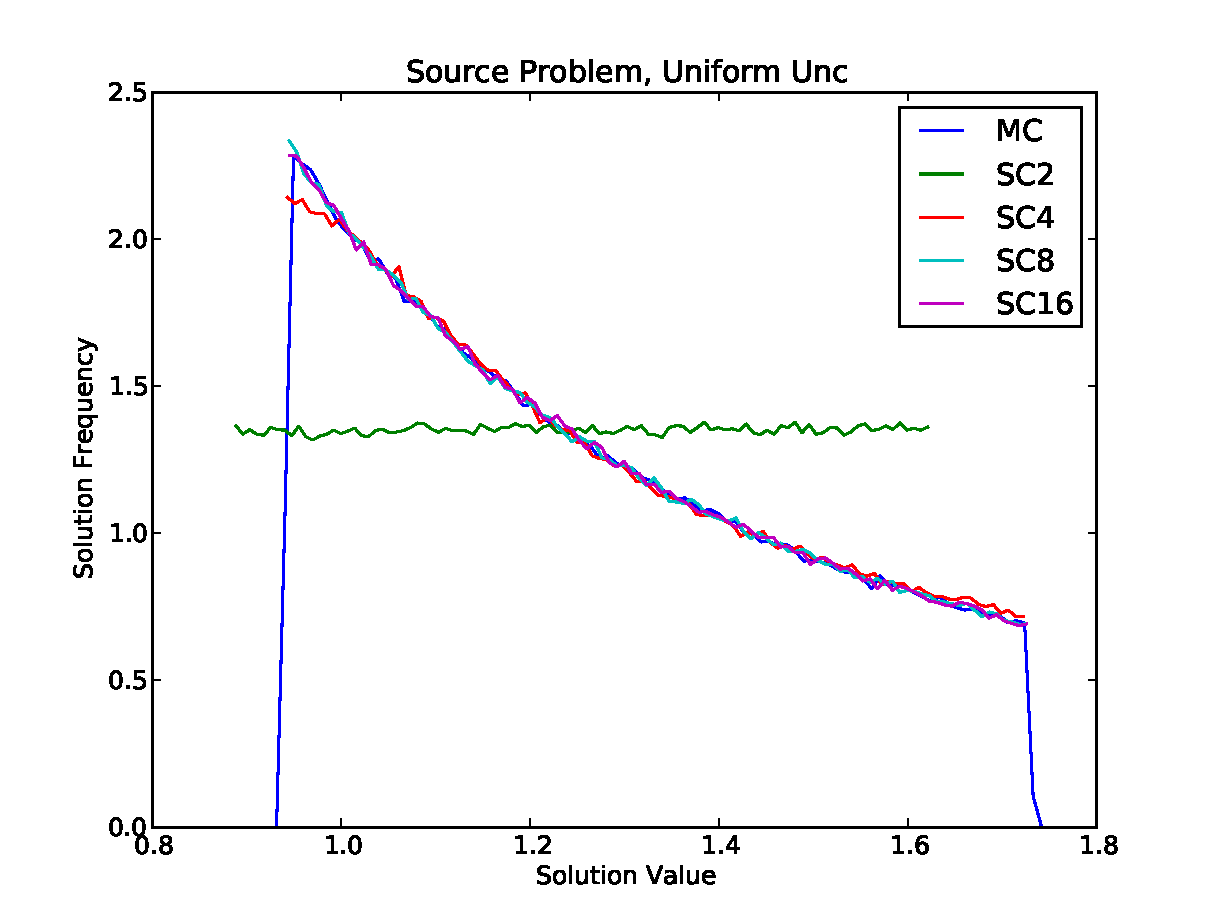
\includegraphics[width=\textwidth]{../graphics/source_uniform_pdfs}
   \caption{Uniform PDFs}
      \label{uni}
  \end{subfigure}
  \begin{subfigure}[b]{0.45\textwidth}
   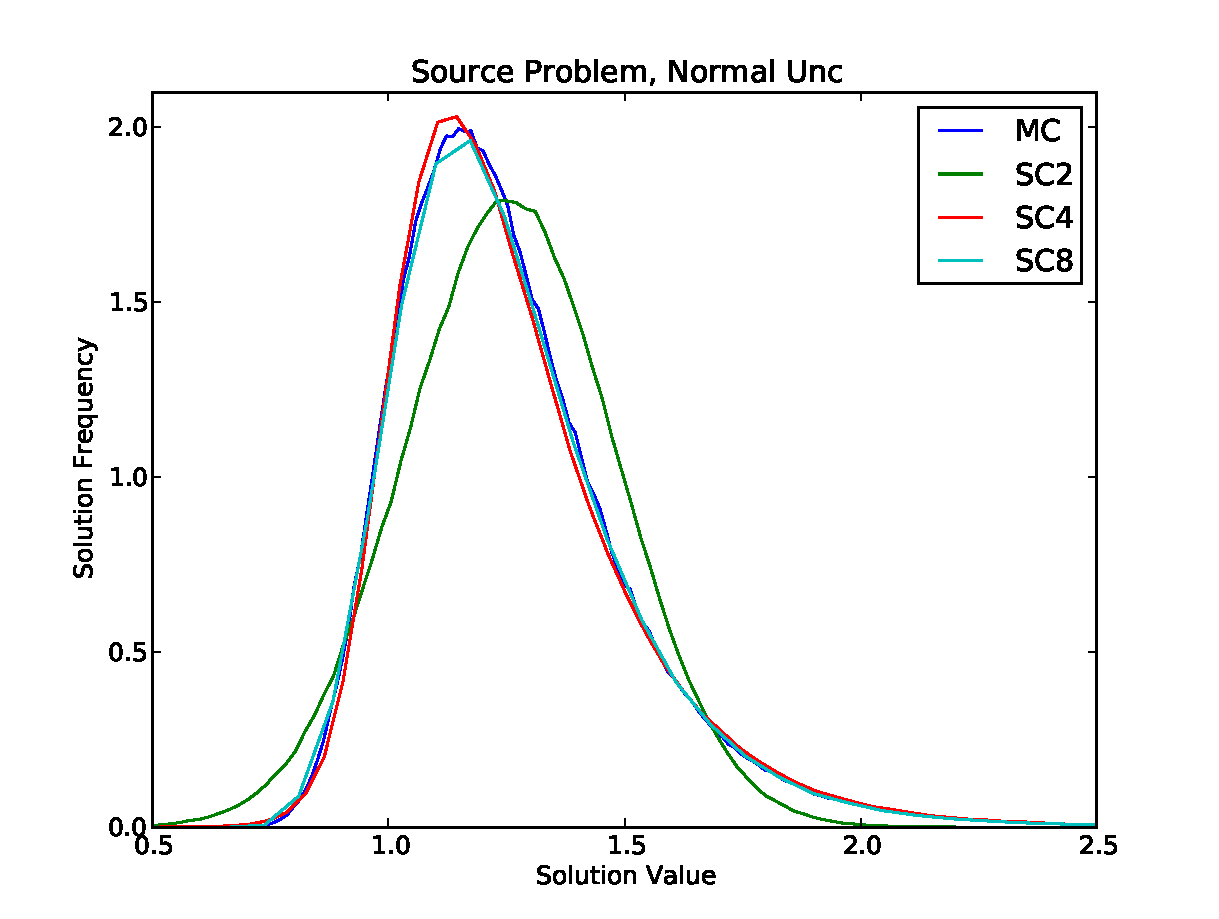
\includegraphics[width=\textwidth]{../graphics/source_normal_pdfs}
   \caption{Normal PDFs}
      \label{norm}
  \end{subfigure}
\caption{Source Problem Solution Distributions}
\label{fig:sourcepdfs}
\end{figure}

The PDFs were obtained by Monte Carlo sampling of the polynomial expansion for the SC cases, and obtained directly for the Monte Carlo case, shown in Fig. \ref{fig:sourcepdfs}.  The x-axis is the value of the scalar flux, and the y-axis is the probability of obtaining a particular flux.


%\begin{table}
%\begin{center}
%\begin{tabular}{c c|l l| r}
%type & runs/order & mean & variance & run time (sec) \\ \hline
%MC & 1\times10^6 &  &  & \\
%SC & 2 & & & \\
%SC & 4 & & & \\
%SC & 8 & & & \\
%SC & 16 & & &
%\end{tabular}
%\end{center}
%\caption{}
%\label{}
%\end{table}
%
%\begin{figure}[h!]
%\centering
%   \includegraphics[width=\textwidth]{../graphics/}
%   \label{}
%   \caption{}
%\end{figure}
